%An
\section{Chuyển đổi từ Mô hình Quan niệm sang Lược đồ Logic}

Dựa trên sơ đồ thực thể kết nối (ERD) và các quy tắc nghiệp vụ đã phân tích ở chương trước, tiến hành chuyển đổi mô hình thực thể quan niệm sang mô hình quan hệ (Relational Schema). Quá trình này được thực hiện thông qua việc áp dụng nghiêm ngặt lý thuyết chuẩn hóa cơ sở dữ liệu (đảm bảo đạt tối thiểu chuẩn 3NF dựa trên tập phủ tối thiểu của các phụ thuộc hàm) nhằm loại bỏ hoàn toàn dư thừa dữ liệu, triệt tiêu các dị thường khi thêm, xóa, sửa, đồng thời đảm bảo tính toàn vẹn tham chiếu và tối ưu hóa hiệu năng truy vấn cho toàn bộ hệ thống quản lý hạ tầng Mini Data Center.

Quá trình chuyển đổi từ các thực thể, thuộc tính và mối quan hệ sang cấu trúc bảng quan hệ tuân thủ các nguyên tắc thiết kế hiện đại: sử dụng khóa chính dạng định danh duy nhất (UUID/$\text{VARCHAR}(36)$) cho toàn bộ các thực thể cốt lõi, áp dụng kiểu dữ liệu tối ưu cho từng loại thuộc tính ($\text{DATETIME}$, $\text{FLOAT}$, $\text{TEXT}$), chuẩn hóa quy tắc đặt tên theo chuẩn PascalCase, và thiết lập đầy đủ các ràng buộc khóa ngoại ($\text{FK}$) nhằm duy trì tính liên kết chặt chẽ giữa các bảng.

Các bảng dữ liệu trong hệ thống được phân rã, tổ chức và phân nhóm thành các phân hệ chức năng chi tiết sau:

\begin{itemize}[leftmargin=2em]
    \item \textbf{Phân hệ Hạ tầng \& Không gian Vật lý:} 
    Quản lý phân cấp không gian và thiết bị từ cấp độ vị trí trung tâm (\texttt{Site}), phòng máy chuyên dụng (\texttt{Room}), tủ chứa thiết bị (\texttt{Rack}) cho đến thiết bị máy chủ vật lý (\texttt{Server}) và các dịch vụ ảo hóa, container chạy trên nền tảng đó (\texttt{Workload}). Việc thiết kế chuỗi liên kết khóa ngoại từ $\text{Site} \to \text{Room} \to \text{Rack} \to \text{Server} \to \text{Workload}$ giúp ánh xạ chính xác sơ đồ vị trí và cấu trúc phân cấp vật lý thực tế vào mô hình dữ liệu quan hệ, hỗ trợ việc tra cứu và quản lý tài nguyên hạ tầng một cách trực quan.

    \item \textbf{Phân hệ Giám sát \& Vận hành Hệ thống:} 
    Chịu trách nhiệm lưu trữ chuỗi thời gian của các chỉ số hiệu năng phần cứng theo thời gian thực như mức độ sử dụng CPU, RAM, lưu lượng mạng và trạng thái container (\texttt{TelemetryMetric}). Đồng thời, phân hệ này quản lý việc thiết lập các ngưỡng cảnh báo động (\texttt{AlertThreshold}), ghi nhận các sự kiện cảnh báo phát sinh (\texttt{Alert}), sự cố hệ thống trầm trọng (\texttt{Incident}) và theo dõi toàn bộ vòng đời xử lý nghiệp vụ bảo trì từ khâu lập phiếu, phân công kỹ thuật viên cho đến khi hoàn tất (\texttt{MaintainTicket}, \texttt{MaintenanceLog}), kết hợp ghi nhận các phiên thao tác thực tế qua kính thực tế ảo tăng cường (\text{ARSessionUsed}).

    \item \textbf{Phân hệ Quản lý Tài sản \& Bảo hành:} 
    Quản lý toàn bộ vòng đời của thiết bị phần cứng thông qua danh mục phân loại tài sản (\texttt{AssetCategory}), bảng thông tin chi tiết tài sản liên kết với máy chủ hoặc thiết bị độc lập (\texttt{Asset}), theo dõi thông tin hợp đồng bảo hành với nhà cung cấp, thời hạn hiệu lực và cấu hình cảnh báo trước hạn (\texttt{Warranty}), cùng bảng ghi nhận lịch sử biến động trạng thái tài sản theo thời gian (\texttt{AssetStatusChange}) để phục vụ công tác kiểm kê và thanh lý.

    \item \textbf{Phân hệ Bảo mật, Phân quyền \& Kiểm toán:} 
    Đảm bảo tính an toàn, phân quyền truy cập chặt chẽ và khả năng truy vết hệ thống thông qua bảng quản lý thông tin tài khoản người dùng (\texttt{User}), định nghĩa các vai trò chức năng trong hệ thống (\texttt{Role}), bảng liên kết nhiều-nhiều quản lý phân quyền người dùng (\texttt{UserRole}) và cơ chế ghi vết nhật ký kiểm toán toàn cục (\texttt{AuditLog}) lưu lại mọi thao tác quan trọng kèm theo địa chỉ IP và mã thực thể tác động.
\end{itemize}

Thông qua quá trình chuẩn hóa và hiện thực hóa tường minh các mối quan hệ kết nối dạng một - nhiều ($1 - N$) từ sơ đồ ERD, mô hình quan hệ đã thiết lập một nền tảng vững chắc, đảm bảo tính nhất quán dữ liệu cao, sẵn sàng cho việc triển khai mã nguồn và xây dựng các câu lệnh truy vấn tối ưu ở các giai đoạn tiếp theo của đồ án.

\subsection{Sơ đồ Lược đồ Quan hệ (Relational Schema Diagram)}

\begin{figure}[H]
    \centering
    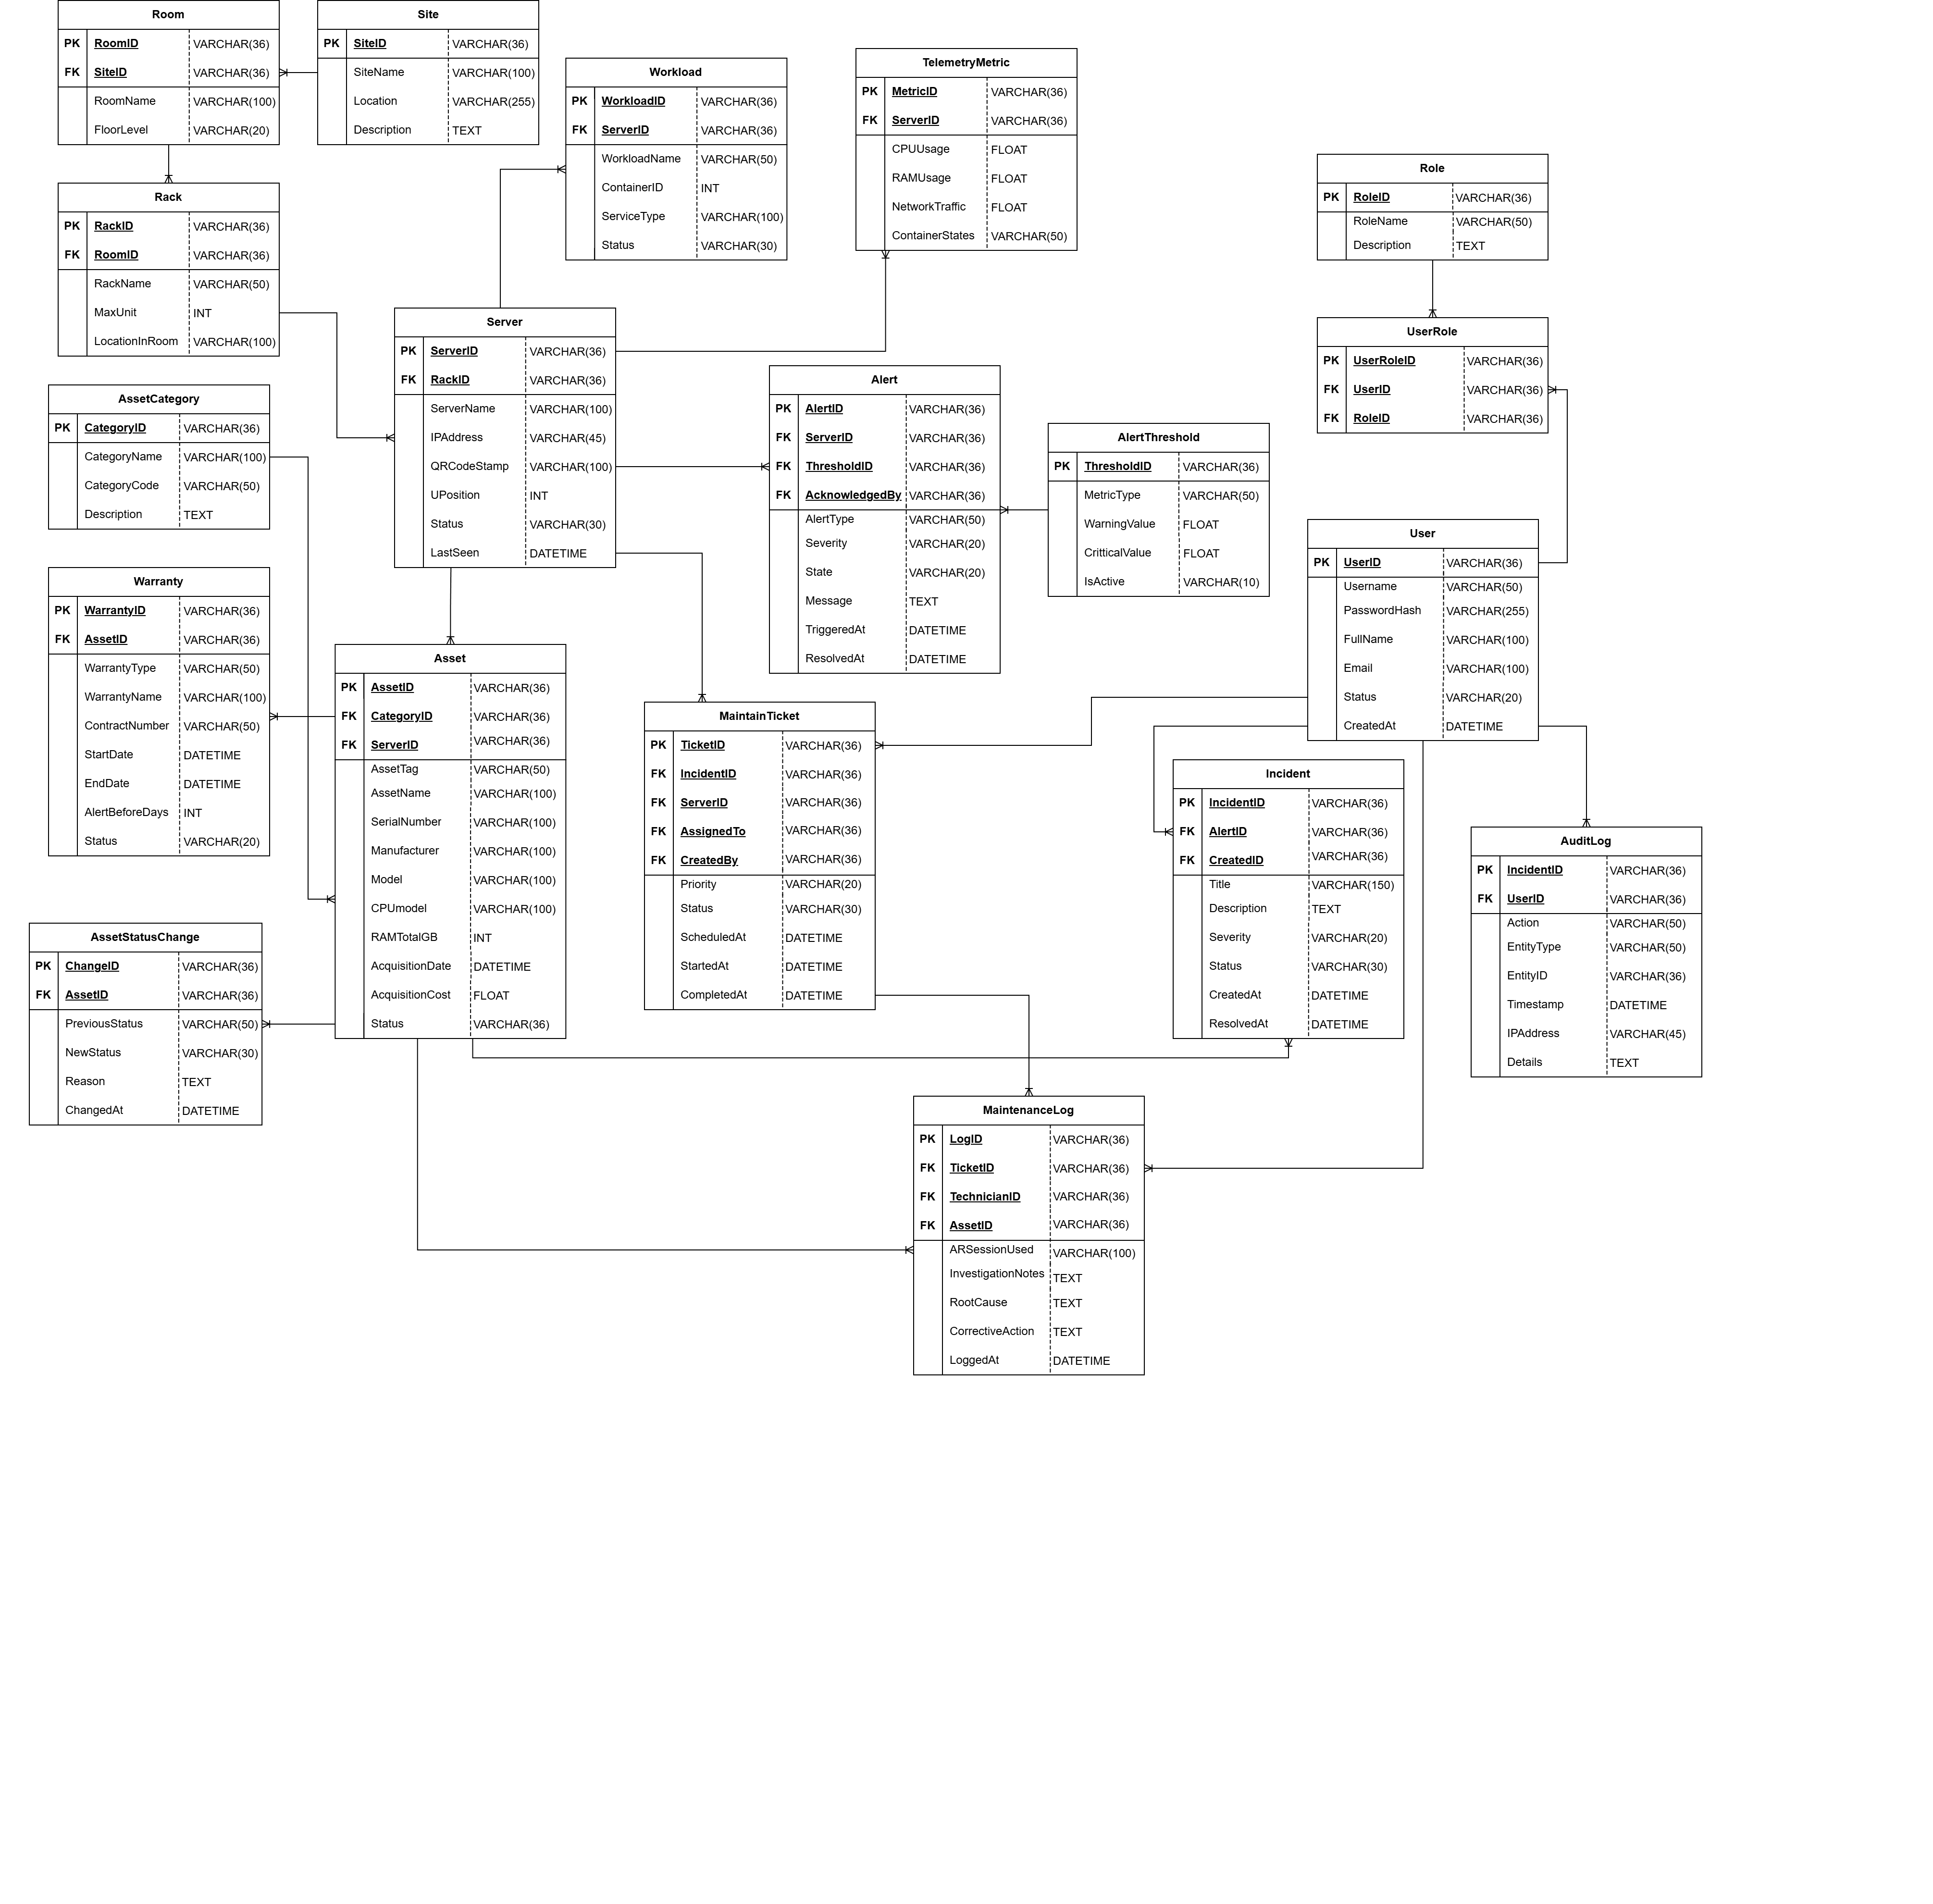
\includegraphics[width=1.0\textwidth]{images/relational_schema.png} 
    \caption{Lược đồ Quan hệ chi tiết hệ thống Quản lý Mini Data Center}
    \label{fig:relational_schema}
\end{figure}
